\section*{Lecture 2: Information and Decision Modeling}

% --- slide page ---
\clearpage
\thispagestyle{empty}
\noindent\textbf{Lecture 2 / Slide 001: Platzhalter für Bild, Bild auf Titelfolie hinter das Logo einsetzen}\hfill {\scriptsize source: 3DM\_02\_Information-and-Decision-Modeling\_SS26.pdf}\par
\vspace{1mm}
\noindent\makebox[\textwidth][c]{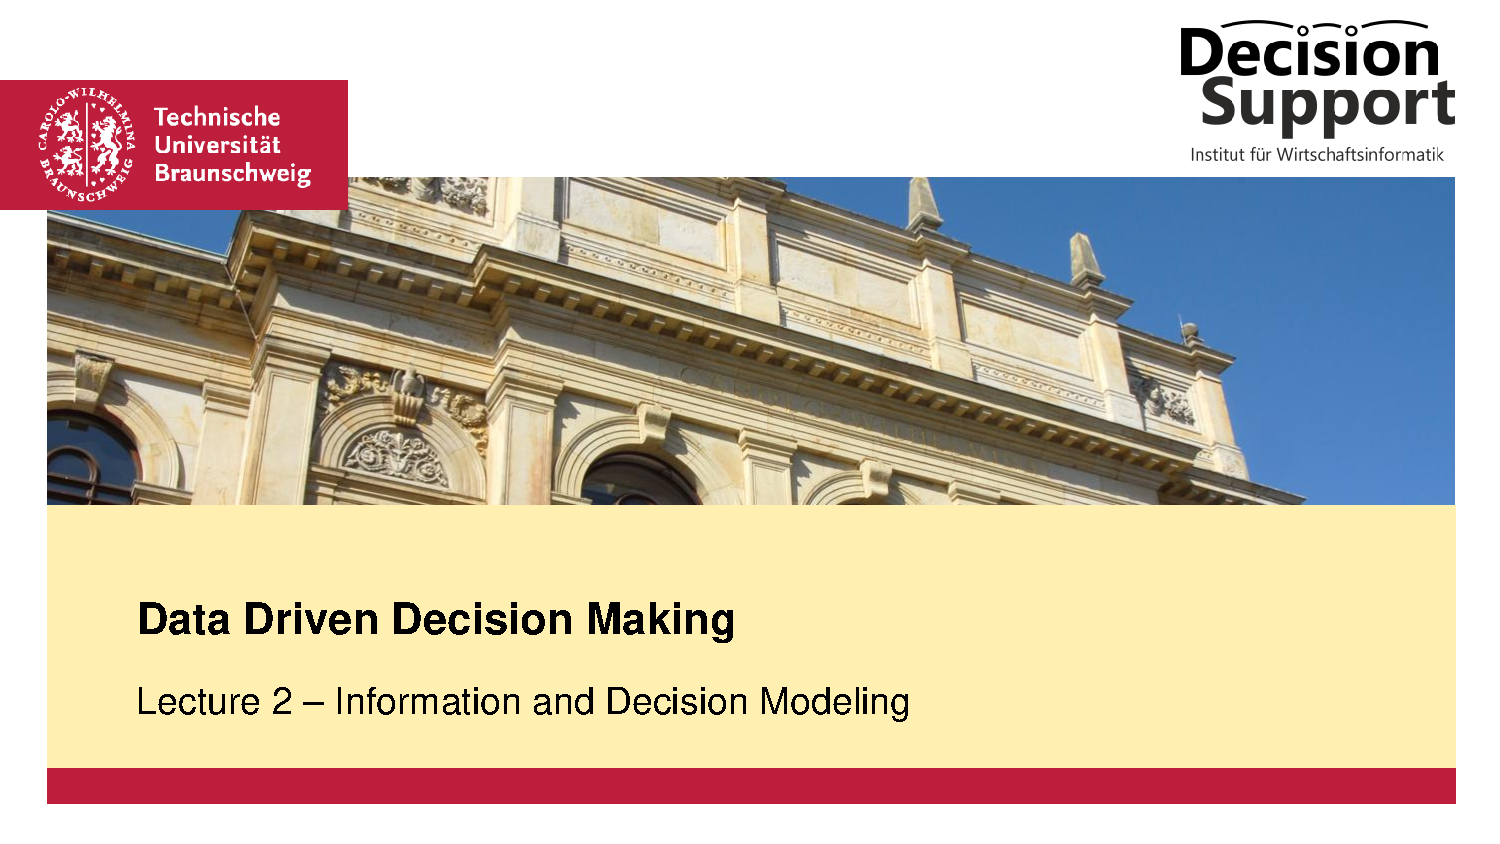
\includegraphics[page=1,width=\textwidth,height=0.455\textheight,keepaspectratio]{../Materials/2026/3DM_02_Information-and-Decision-Modeling_SS26.pdf}}
\vspace{1mm}
\begin{minipage}[t][0.47\textheight][t]{\textwidth}
\scriptsize
\setlength{\parskip}{1.2pt}
\begin{multicols}{2}
\noindent\textbf{日本語訳・要約}\; 表紙。第2回はInformation Modeling and Decision Modelingを扱う。\par

\noindent\textbf{解説}\; 第1回の意思決定ループを具体化し、現実データをどのような情報モデルにし、どのような決定モデルで解くかを学ぶ。\par

\noindent\textbf{試験ポイント}\; Lecture 2は過去問頻出。特にBAプロセス、時間依存旅行時間、FIFO、ヒューリスティックが重要。\par

\noindent\textbf{過去問関連}\; SS24 Aufgabe 1a, WS23/24 Aufgabe 2, WS23/24 Aufgabe 3, WS22/23 Aufgabe 4, WS23/24 Aufgabe 4-5, SS25 Exercise 2 と広く関連。\par

\noindent\textbf{確認問題}\; 情報モデルと決定モデルの違いを一文で説明せよ。\par

\end{multicols}
\end{minipage}
% --- slide page ---
\clearpage
\thispagestyle{empty}
\noindent\textbf{Lecture 2 / Slide 002: Goals of today‘s lecture}\hfill {\scriptsize source: 3DM\_02\_Information-and-Decision-Modeling\_SS26.pdf}\par
\vspace{1mm}
\noindent\makebox[\textwidth][c]{\includegraphics[page=2,width=\textwidth,height=0.455\textheight,keepaspectratio]{../Materials/2026/3DM_02_Information-and-Decision-Modeling_SS26.pdf}}
\vspace{1mm}
\begin{minipage}[t][0.47\textheight][t]{\textwidth}
\scriptsize
\setlength{\parskip}{1.2pt}
\begin{multicols}{2}
\noindent\textbf{日本語訳・要約}\; 本日の目標は、Business Analyticsのプロセス、情報・意思決定モデル、時間依存旅行時間付きTSP、TSP解法を理解すること。\par

\noindent\textbf{解説}\; 講義前半は概念、後半は移動時間データを使ったケーススタディ。\par

\noindent\textbf{試験ポイント}\; データ収集から意思決定までの流れを、TSP例で具体化できるようにする。\par

\noindent\textbf{過去問関連}\; WS22/23 Aufgabe 2-3, WS23/24 Aufgabe 1-3, WS22/23 Aufgabe 4, WS23/24 Aufgabe 4-5, SS25 Exercise 2 と関連。\par

\noindent\textbf{確認問題}\; 今日の講義の中心的なケーススタディは何か。\par

\end{multicols}
\end{minipage}
% --- slide page ---
\clearpage
\thispagestyle{empty}
\noindent\textbf{Lecture 2 / Slide 003: Agenda}\hfill {\scriptsize source: 3DM\_02\_Information-and-Decision-Modeling\_SS26.pdf}\par
\vspace{1mm}
\noindent\makebox[\textwidth][c]{\includegraphics[page=3,width=\textwidth,height=0.455\textheight,keepaspectratio]{../Materials/2026/3DM_02_Information-and-Decision-Modeling_SS26.pdf}}
\vspace{1mm}
\begin{minipage}[t][0.47\textheight][t]{\textwidth}
\scriptsize
\setlength{\parskip}{1.2pt}
\begin{multicols}{2}
\noindent\textbf{日本語訳・要約}\; アジェンダは、Information/Decision Modelingと、時間依存旅行時間付きTSPのケーススタディ。\par

\noindent\textbf{解説}\; 抽象フレームを先に学び、その後で都市交通データへの適用を見る。\par

\noindent\textbf{試験ポイント}\; 試験では定義だけでなく、ケースへ対応付ける力が問われる。\par

\noindent\textbf{過去問関連}\; WS22/23 Aufgabe 2-3, WS23/24 Aufgabe 1-3, WS23/24 Aufgabe 3 と関連。\par

\noindent\textbf{確認問題}\; 抽象モデルとケーススタディの関係を説明せよ。\par

\end{multicols}
\end{minipage}
% --- slide page ---
\clearpage
\thispagestyle{empty}
\noindent\textbf{Lecture 2 / Slide 004: Decision making}\hfill {\scriptsize source: 3DM\_02\_Information-and-Decision-Modeling\_SS26.pdf}\par
\vspace{1mm}
\noindent\makebox[\textwidth][c]{\includegraphics[page=4,width=\textwidth,height=0.455\textheight,keepaspectratio]{../Materials/2026/3DM_02_Information-and-Decision-Modeling_SS26.pdf}}
\vspace{1mm}
\begin{minipage}[t][0.47\textheight][t]{\textwidth}
\scriptsize
\setlength{\parskip}{1.2pt}
\begin{multicols}{2}
\noindent\textbf{日本語訳・要約}\; 意思決定ループ。現実世界で行動が実行され状態が観測される。Aggregationは現実データを情報モデルの次元に移す。Information Modelは情報を凝縮して表現する。Decision Modelは決定空間を定義し評価する。Implementationは解を現実の行動へ戻す。\par

\noindent\textbf{解説}\; Real-World -> Aggregation -> Information Model -> Decision Model -> Implementation -> Real-World の流れを説明できることが最重要。\par

\noindent\textbf{試験ポイント}\; AggregationとImplementationを混同しない。情報モデルは「何を知っているか」、決定モデルは「何を選び、どう評価するか」。\par

\noindent\textbf{過去問関連}\; SS24 Aufgabe 1a, WS23/24 Aufgabe 2, WS23/24 Aufgabe 3 と強く関連。SS24 Aufgabe 1aでは各機能の説明が問われた。\par

\noindent\textbf{確認問題}\; Aggregation, Information Model, Decision Model, Implementationをそれぞれ定義せよ。\par

\end{multicols}
\end{minipage}
% --- slide page ---
\clearpage
\thispagestyle{empty}
\noindent\textbf{Lecture 2 / Slide 005: Selection of information and decision model}\hfill {\scriptsize source: 3DM\_02\_Information-and-Decision-Modeling\_SS26.pdf}\par
\vspace{1mm}
\noindent\makebox[\textwidth][c]{\includegraphics[page=5,width=\textwidth,height=0.455\textheight,keepaspectratio]{../Materials/2026/3DM_02_Information-and-Decision-Modeling_SS26.pdf}}
\vspace{1mm}
\begin{minipage}[t][0.47\textheight][t]{\textwidth}
\scriptsize
\setlength{\parskip}{1.2pt}
\begin{multicols}{2}
\noindent\textbf{日本語訳・要約}\; 情報モデルと決定モデルは初期仮説に基づいて設計される。仮説は現実問題の観察やデータから生まれ、分析結果により仮説が確認・修正される。\par

\noindent\textbf{解説}\; モデル化は固定的なものではなく、descriptive analyticsで現実を観察し、prescriptive analyticsで意思決定へつなぐ反復プロセスである。\par

\noindent\textbf{試験ポイント}\; 情報モデルの選択は仮説依存。例えば「旅行時間は一定」という仮説が崩れれば時間依存モデルへ変える。\par

\noindent\textbf{過去問関連}\; WS22/23 Aufgabe 2-3, WS23/24 Aufgabe 1-3, SS24 Aufgabe 1b と関連。\par

\noindent\textbf{確認問題}\; 観測データが初期仮説を否定した場合、モデル化では何をするか。\par

\end{multicols}
\end{minipage}
% --- slide page ---
\clearpage
\thispagestyle{empty}
\noindent\textbf{Lecture 2 / Slide 006: task}\hfill {\scriptsize source: 3DM\_02\_Information-and-Decision-Modeling\_SS26.pdf}\par
\vspace{1mm}
\noindent\makebox[\textwidth][c]{\includegraphics[page=6,width=\textwidth,height=0.455\textheight,keepaspectratio]{../Materials/2026/3DM_02_Information-and-Decision-Modeling_SS26.pdf}}
\vspace{1mm}
\begin{minipage}[t][0.47\textheight][t]{\textwidth}
\scriptsize
\setlength{\parskip}{1.2pt}
\begin{multicols}{2}
\noindent\textbf{日本語訳・要約}\; タスク、問題構造、記録データ、探索、対象データの関係を示す図。\par

\noindent\textbf{解説}\; 現実問題の構造を理解し、記録されたデータから意思決定に必要なデータを探す流れを表す。\par

\noindent\textbf{試験ポイント}\; データはそのまま意思決定に使えるとは限らず、構造理解と抽出・変換が必要。\par

\noindent\textbf{過去問関連}\; WS22/23 Aufgabe 2-3, WS23/24 Aufgabe 1-3 と関連。BAプロセス図の説明に使える。\par

\noindent\textbf{確認問題}\; recorded data と target data の違いは何か。\par

\end{multicols}
\end{minipage}
% --- slide page ---
\clearpage
\thispagestyle{empty}
\noindent\textbf{Lecture 2 / Slide 007: Planning of Mobility/Transp.: From Structure to Appearance}\hfill {\scriptsize source: 3DM\_02\_Information-and-Decision-Modeling\_SS26.pdf}\par
\vspace{1mm}
\noindent\makebox[\textwidth][c]{\includegraphics[page=7,width=\textwidth,height=0.455\textheight,keepaspectratio]{../Materials/2026/3DM_02_Information-and-Decision-Modeling_SS26.pdf}}
\vspace{1mm}
\begin{minipage}[t][0.47\textheight][t]{\textwidth}
\scriptsize
\setlength{\parskip}{1.2pt}
\begin{multicols}{2}
\noindent\textbf{日本語訳・要約}\; 現実の意思決定問題は数理モデル化に合わせて単純化される。単純化の過程で情報の構造と外見を切り分ける。\par

\noindent\textbf{解説}\; Meisel/Mattfeldの視点では、ORとData Mining/IDAは現実問題の構造化とデータ活用で相補的に働く。\par

\noindent\textbf{試験ポイント}\; どの情報を残し、どの情報を捨てるかが情報モデル設計の中心。\par

\noindent\textbf{過去問関連}\; WS22/23 Aufgabe 2-3, WS23/24 Aufgabe 1-3, WS23/24 Aufgabe 1 と関連。\par

\noindent\textbf{確認問題}\; 数理モデル化のために現実問題を単純化する利点と危険は何か。\par

\end{multicols}
\end{minipage}
% --- slide page ---
\clearpage
\thispagestyle{empty}
\noindent\textbf{Lecture 2 / Slide 008: Unified View of IDA and PMT}\hfill {\scriptsize source: 3DM\_02\_Information-and-Decision-Modeling\_SS26.pdf}\par
\vspace{1mm}
\noindent\makebox[\textwidth][c]{\includegraphics[page=8,width=\textwidth,height=0.455\textheight,keepaspectratio]{../Materials/2026/3DM_02_Information-and-Decision-Modeling_SS26.pdf}}
\vspace{1mm}
\begin{minipage}[t][0.47\textheight][t]{\textwidth}
\scriptsize
\setlength{\parskip}{1.2pt}
\begin{multicols}{2}
\noindent\textbf{日本語訳・要約}\; IDAとPMTの統一ビュー。goal, problem, structure, search, decision という流れで、データ分析と意思決定を接続する。\par

\noindent\textbf{解説}\; IDAはデータからパターンや構造を抽出し、PMT/ORはそれを使って意思決定をモデル化・解決する。\par

\noindent\textbf{試験ポイント}\; Business Analyticsを「データ分析」「統計」「OR/意思決定」の接続として説明できるようにする。\par

\noindent\textbf{過去問関連}\; WS22/23 Aufgabe 2-3, WS23/24 Aufgabe 1-3 と強く関連。WS22/23 Aufgabe 2, WS23/24 Aufgabe 1でBA分野が問われた。\par

\noindent\textbf{確認問題}\; IDAとPMTはBusiness Analyticsの中でどう接続するか。\par

\end{multicols}
\end{minipage}
% --- slide page ---
\clearpage
\thispagestyle{empty}
\noindent\textbf{Lecture 2 / Slide 009: Example: Traveling Salesperson Problem}\hfill {\scriptsize source: 3DM\_02\_Information-and-Decision-Modeling\_SS26.pdf}\par
\vspace{1mm}
\noindent\makebox[\textwidth][c]{\includegraphics[page=9,width=\textwidth,height=0.455\textheight,keepaspectratio]{../Materials/2026/3DM_02_Information-and-Decision-Modeling_SS26.pdf}}
\vspace{1mm}
\begin{minipage}[t][0.47\textheight][t]{\textwidth}
\scriptsize
\setlength{\parskip}{1.2pt}
\begin{multicols}{2}
\noindent\textbf{日本語訳・要約}\; TSP例。仮説は旅行時間が一定であること。情報モデルは旅行時間行列、決定モデルはTSP。出力は顧客訪問順序である。\par

\noindent\textbf{解説}\; このページは情報モデルと決定モデルの最小例。後に時間依存・不確実性・動的性を加える基準点になる。\par

\noindent\textbf{試験ポイント}\; travel time matrixとTSPモデルを区別する。仮説が変わると情報モデルも決定モデルも変わる可能性がある。\par

\noindent\textbf{過去問関連}\; WS22/23 Aufgabe 1, WS23/24 Aufgabe 3, SS24 Aufgabe 1b と関連。\par

\noindent\textbf{確認問題}\; TSP例で、仮説・情報モデル・決定モデル・出力を対応させよ。\par

\end{multicols}
\end{minipage}
% --- slide page ---
\clearpage
\thispagestyle{empty}
\noindent\textbf{Lecture 2 / Slide 010: Agenda}\hfill {\scriptsize source: 3DM\_02\_Information-and-Decision-Modeling\_SS26.pdf}\par
\vspace{1mm}
\noindent\makebox[\textwidth][c]{\includegraphics[page=10,width=\textwidth,height=0.455\textheight,keepaspectratio]{../Materials/2026/3DM_02_Information-and-Decision-Modeling_SS26.pdf}}
\vspace{1mm}
\begin{minipage}[t][0.47\textheight][t]{\textwidth}
\scriptsize
\setlength{\parskip}{1.2pt}
\begin{multicols}{2}
\noindent\textbf{日本語訳・要約}\; ケーススタディへ移る。対象は時間依存旅行時間をもつTSPである。\par

\noindent\textbf{解説}\; 静的TSPから、出発時刻により移動時間が変わるTSPへ拡張する。\par

\noindent\textbf{試験ポイント}\; 時間依存性があると、移動コストはアークだけでなく出発時刻にも依存する。\par

\noindent\textbf{過去問関連}\; WS22/23 Aufgabe 4, WS23/24 Aufgabe 4-5, SS25 Exercise 2 と関連。\par

\noindent\textbf{確認問題}\; 時間依存TSPではコスト関数は何に依存するか。\par

\end{multicols}
\end{minipage}
% --- slide page ---
\clearpage
\thispagestyle{empty}
\noindent\textbf{Lecture 2 / Slide 011: Motivation}\hfill {\scriptsize source: 3DM\_02\_Information-and-Decision-Modeling\_SS26.pdf}\par
\vspace{1mm}
\noindent\makebox[\textwidth][c]{\includegraphics[page=11,width=\textwidth,height=0.455\textheight,keepaspectratio]{../Materials/2026/3DM_02_Information-and-Decision-Modeling_SS26.pdf}}
\vspace{1mm}
\begin{minipage}[t][0.47\textheight][t]{\textwidth}
\scriptsize
\setlength{\parskip}{1.2pt}
\begin{multicols}{2}
\noindent\textbf{日本語訳・要約}\; サービスルーティングでは高価な運転時間を節約し、顧客サービスを改善し、資源を効率的に使うことが重要である。\par

\noindent\textbf{解説}\; 交通・配送では少しの移動時間改善がコストやサービス品質へ大きく影響する。\par

\noindent\textbf{試験ポイント}\; 目的関数は総移動時間だけでなく、遅延・サービス品質・資源利用も関係しうる。\par

\noindent\textbf{過去問関連}\; WS22/23 Aufgabe 1, WS23/24 Aufgabe 3, SS24 Aufgabe 1b と関連。\par

\noindent\textbf{確認問題}\; サービスルーティングで移動時間が重要な理由を説明せよ。\par

\end{multicols}
\end{minipage}
% --- slide page ---
\clearpage
\thispagestyle{empty}
\noindent\textbf{Lecture 2 / Slide 012: Time-Dependent Travel Times}\hfill {\scriptsize source: 3DM\_02\_Information-and-Decision-Modeling\_SS26.pdf}\par
\vspace{1mm}
\noindent\makebox[\textwidth][c]{\includegraphics[page=12,width=\textwidth,height=0.455\textheight,keepaspectratio]{../Materials/2026/3DM_02_Information-and-Decision-Modeling_SS26.pdf}}
\vspace{1mm}
\begin{minipage}[t][0.47\textheight][t]{\textwidth}
\scriptsize
\setlength{\parskip}{1.2pt}
\begin{multicols}{2}
\noindent\textbf{日本語訳・要約}\; 旅行時間は時間と空間で変動する。道路セグメントごとに異なる旅行時間があり、天候、事故、曜日、時間帯などで変わる。\par

\noindent\textbf{解説}\; 時間依存旅行時間の情報モデルは、単なる顧客間距離ではなく、道路セグメント・時間帯・速度/移動時間を含む。\par

\noindent\textbf{試験ポイント}\; 時間変動と空間変動を分けて説明する。\par

\noindent\textbf{過去問関連}\; WS22/23 Aufgabe 4, WS23/24 Aufgabe 4-5, SS25 Exercise 2 と関連。\par

\noindent\textbf{確認問題}\; 旅行時間が時間と空間で変動するとはどういう意味か。\par

\end{multicols}
\end{minipage}
% --- slide page ---
\clearpage
\thispagestyle{empty}
\noindent\textbf{Lecture 2 / Slide 013: Modeling (sketched)}\hfill {\scriptsize source: 3DM\_02\_Information-and-Decision-Modeling\_SS26.pdf}\par
\vspace{1mm}
\noindent\makebox[\textwidth][c]{\includegraphics[page=13,width=\textwidth,height=0.455\textheight,keepaspectratio]{../Materials/2026/3DM_02_Information-and-Decision-Modeling_SS26.pdf}}
\vspace{1mm}
\begin{minipage}[t][0.47\textheight][t]{\textwidth}
\scriptsize
\setlength{\parskip}{1.2pt}
\begin{multicols}{2}
\noindent\textbf{日本語訳・要約}\; 情報モデルは、顧客間の時間依存旅行時間、時間依存旅行時間行列または複数行列。決定モデルは旅行時間最小化、全顧客訪問、ルーティング制約、時刻に依存する顧客間移動決定変数を含む。\par

\noindent\textbf{解説}\; 時間依存性を入れると、同じiからjへの移動でも出発時刻でコストが変わる。\par

\noindent\textbf{試験ポイント}\; 情報モデルと決定モデルの要素を答案で列挙できること。\par

\noindent\textbf{過去問関連}\; WS22/23 Aufgabe 4, WS23/24 Aufgabe 4-5, SS25 Exercise 2, WS22/23 Aufgabe 1 と関連。\par

\noindent\textbf{確認問題}\; 時間依存旅行時間TSPの情報モデルと決定モデルを分けて書け。\par

\end{multicols}
\end{minipage}
% --- slide page ---
\clearpage
\thispagestyle{empty}
\noindent\textbf{Lecture 2 / Slide 014: Data Collection: Floating Car Data}\hfill {\scriptsize source: 3DM\_02\_Information-and-Decision-Modeling\_SS26.pdf}\par
\vspace{1mm}
\noindent\makebox[\textwidth][c]{\includegraphics[page=14,width=\textwidth,height=0.455\textheight,keepaspectratio]{../Materials/2026/3DM_02_Information-and-Decision-Modeling_SS26.pdf}}
\vspace{1mm}
\begin{minipage}[t][0.47\textheight][t]{\textwidth}
\scriptsize
\setlength{\parskip}{1.2pt}
\begin{multicols}{2}
\noindent\textbf{日本語訳・要約}\; Floating Car Dataは、時間・道路セグメントごとの旅行時間を得るデータである。十分なデータ量が必要で、オンデマンド型の情報として活用される。\par

\noindent\textbf{解説}\; FCDはタクシーや車両から得られる移動観測データ。生データから速度・リンク・時間帯を推定して情報モデルを作る。\par

\noindent\textbf{試験ポイント}\; データ収集 -> クリーニング -> 集約 -> 一般化という流れを説明する。\par

\noindent\textbf{過去問関連}\; WS22/23 Aufgabe 4 と関連。過去交通観測から時間帯別平均旅行時間を作る手順が問われた。\par

\noindent\textbf{確認問題}\; FCDから旅行時間行列を作るにはどの処理が必要か。\par

\end{multicols}
\end{minipage}
% --- slide page ---
\clearpage
\thispagestyle{empty}
\noindent\textbf{Lecture 2 / Slide 015: FCD-Collection und Use}\hfill {\scriptsize source: 3DM\_02\_Information-and-Decision-Modeling\_SS26.pdf}\par
\vspace{1mm}
\noindent\makebox[\textwidth][c]{\includegraphics[page=15,width=\textwidth,height=0.455\textheight,keepaspectratio]{../Materials/2026/3DM_02_Information-and-Decision-Modeling_SS26.pdf}}
\vspace{1mm}
\begin{minipage}[t][0.47\textheight][t]{\textwidth}
\scriptsize
\setlength{\parskip}{1.2pt}
\begin{multicols}{2}
\noindent\textbf{日本語訳・要約}\; FCDの収集と利用には、タクシーフリート、ディスパッチャ、公共交通管理、プロバイダ、インターネットなどが関係する。\par

\noindent\textbf{解説}\; データは複数主体を通じて集まる。データの粒度や欠損は後のモデル品質に影響する。\par

\noindent\textbf{試験ポイント}\; 誰がデータを持ち、どの形で意思決定に使えるかを考える。\par

\noindent\textbf{過去問関連}\; WS22/23 Aufgabe 4のデータ取得手順の背景。\par

\noindent\textbf{確認問題}\; FCDのデータ提供者と利用者を挙げよ。\par

\end{multicols}
\end{minipage}
% --- slide page ---
\clearpage
\thispagestyle{empty}
\noindent\textbf{Lecture 2 / Slide 016: Floating Car Data: Speed Calculation}\hfill {\scriptsize source: 3DM\_02\_Information-and-Decision-Modeling\_SS26.pdf}\par
\vspace{1mm}
\noindent\makebox[\textwidth][c]{\includegraphics[page=16,width=\textwidth,height=0.455\textheight,keepaspectratio]{../Materials/2026/3DM_02_Information-and-Decision-Modeling_SS26.pdf}}
\vspace{1mm}
\begin{minipage}[t][0.47\textheight][t]{\textwidth}
\scriptsize
\setlength{\parskip}{1.2pt}
\begin{multicols}{2}
\noindent\textbf{日本語訳・要約}\; タクシーデータはそのまま道路、方向、速度を与えないため、必要な手順としてデータの位置合わせ、リンクへの割付、方向判定、速度計算が必要である。\par

\noindent\textbf{解説}\; 生GPSデータは情報モデルではない。地図マッチングと速度推定を通じて道路セグメント別データになる。\par

\noindent\textbf{試験ポイント}\; 生データと意思決定用データの違いを説明する。\par

\noindent\textbf{過去問関連}\; WS22/23 Aufgabe 4 と関連。観測値から旅行時間を作る手順。\par

\noindent\textbf{確認問題}\; Taxi GPSデータをなぜそのまま旅行時間行列にできないか。\par

\end{multicols}
\end{minipage}
% --- slide page ---
\clearpage
\thispagestyle{empty}
\noindent\textbf{Lecture 2 / Slide 017: Floating Car Data: Speed Calculation}\hfill {\scriptsize source: 3DM\_02\_Information-and-Decision-Modeling\_SS26.pdf}\par
\vspace{1mm}
\noindent\makebox[\textwidth][c]{\includegraphics[page=17,width=\textwidth,height=0.455\textheight,keepaspectratio]{../Materials/2026/3DM_02_Information-and-Decision-Modeling_SS26.pdf}}
\vspace{1mm}
\begin{minipage}[t][0.47\textheight][t]{\textwidth}
\scriptsize
\setlength{\parskip}{1.2pt}
\begin{multicols}{2}
\noindent\textbf{日本語訳・要約}\; リンク、時刻、速度の表。観測データを道路リンク単位・時間単位に整理している。\par

\noindent\textbf{解説}\; この表はAggregationの中間成果。個別車両の観測をリンク別速度へ変換する。\par

\noindent\textbf{試験ポイント}\; 列の意味を理解し、後の時間帯別平均やクラスターに接続する。\par

\noindent\textbf{過去問関連}\; WS22/23 Aufgabe 4 と関連。\par

\noindent\textbf{確認問題}\; link, time, speed は情報モデルのどの段階か。\par

\end{multicols}
\end{minipage}
% --- slide page ---
\clearpage
\thispagestyle{empty}
\noindent\textbf{Lecture 2 / Slide 018: Data Analysis}\hfill {\scriptsize source: 3DM\_02\_Information-and-Decision-Modeling\_SS26.pdf}\par
\vspace{1mm}
\noindent\makebox[\textwidth][c]{\includegraphics[page=18,width=\textwidth,height=0.455\textheight,keepaspectratio]{../Materials/2026/3DM_02_Information-and-Decision-Modeling_SS26.pdf}}
\vspace{1mm}
\begin{minipage}[t][0.47\textheight][t]{\textwidth}
\scriptsize
\setlength{\parskip}{1.2pt}
\begin{multicols}{2}
\noindent\textbf{日本語訳・要約}\; 速度パターンは日内で変わり、同じ日・同じ時刻でも変動がある。仮説が確認される一方で、ばらつきも存在する。\par

\noindent\textbf{解説}\; 平均だけでなくばらつきがあるため、Lecture 3の不確実性へつながる。\par

\noindent\textbf{試験ポイント}\; 日内変動と確率的ばらつきを区別する。\par

\noindent\textbf{過去問関連}\; WS22/23 Aufgabe 4, WS23/24 Aufgabe 4-5, SS25 Exercise 2, WS22/23 Aufgabe 5, SS24 Aufgabe 2a, WS24/25 Aufgabe 3 と関連。\par

\noindent\textbf{確認問題}\; 同じ時間帯でも速度がばらつく場合、どの講義テーマにつながるか。\par

\end{multicols}
\end{minipage}
% --- slide page ---
\clearpage
\thispagestyle{empty}
\noindent\textbf{Lecture 2 / Slide 019: link}\hfill {\scriptsize source: 3DM\_02\_Information-and-Decision-Modeling\_SS26.pdf}\par
\vspace{1mm}
\noindent\makebox[\textwidth][c]{\includegraphics[page=19,width=\textwidth,height=0.455\textheight,keepaspectratio]{../Materials/2026/3DM_02_Information-and-Decision-Modeling_SS26.pdf}}
\vspace{1mm}
\begin{minipage}[t][0.47\textheight][t]{\textwidth}
\scriptsize
\setlength{\parskip}{1.2pt}
\begin{multicols}{2}
\noindent\textbf{日本語訳・要約}\; 速度、最大速度、混雑率などを持つデータ。道路リンクごとの交通品質を算出できる。\par

\noindent\textbf{解説}\; 最大速度に対する実際の速度比などを使い、セグメント間で比較可能な指標にする。\par

\noindent\textbf{試験ポイント}\; 正規化や交通品質指標の意味を理解する。\par

\noindent\textbf{過去問関連}\; WS22/23 Aufgabe 4の集約・平均化手順に関連。\par

\noindent\textbf{確認問題}\; maxspeedを使うと何を比較しやすくなるか。\par

\end{multicols}
\end{minipage}
% --- slide page ---
\clearpage
\thispagestyle{empty}
\noindent\textbf{Lecture 2 / Slide 020: Small number of observations}\hfill {\scriptsize source: 3DM\_02\_Information-and-Decision-Modeling\_SS26.pdf}\par
\vspace{1mm}
\noindent\makebox[\textwidth][c]{\includegraphics[page=20,width=\textwidth,height=0.455\textheight,keepaspectratio]{../Materials/2026/3DM_02_Information-and-Decision-Modeling_SS26.pdf}}
\vspace{1mm}
\begin{minipage}[t][0.47\textheight][t]{\textwidth}
\scriptsize
\setlength{\parskip}{1.2pt}
\begin{multicols}{2}
\noindent\textbf{日本語訳・要約}\; 観測数が少ない道路と多い道路がある。空間分布を可視化し、データの偏りを確認する。\par

\noindent\textbf{解説}\; データ量が少ない場所では推定値が不安定。モデル化には補完や一般化が必要になる。\par

\noindent\textbf{試験ポイント}\; データ量の偏りが情報モデルの信頼性へ影響することを説明する。\par

\noindent\textbf{過去問関連}\; SS24 Aufgabe 1b, WS23/24 Aufgabe 6, SS24 Aufgabe 2b, SS25 Exercise 4 と関連。\par

\noindent\textbf{確認問題}\; 観測数が少ないリンクをそのまま使う危険は何か。\par

\end{multicols}
\end{minipage}
% --- slide page ---
\clearpage
\thispagestyle{empty}
\noindent\textbf{Lecture 2 / Slide 021: source: DLR}\hfill {\scriptsize source: 3DM\_02\_Information-and-Decision-Modeling\_SS26.pdf}\par
\vspace{1mm}
\noindent\makebox[\textwidth][c]{\includegraphics[page=21,width=\textwidth,height=0.455\textheight,keepaspectratio]{../Materials/2026/3DM_02_Information-and-Decision-Modeling_SS26.pdf}}
\vspace{1mm}
\begin{minipage}[t][0.47\textheight][t]{\textwidth}
\scriptsize
\setlength{\parskip}{1.2pt}
\begin{multicols}{2}
\noindent\textbf{日本語訳・要約}\; リンクID、時刻、速度などからなるデータ例。個別観測を集約対象として整理している。\par

\noindent\textbf{解説}\; このページも、現実データを情報モデルへ入れる前のデータ構造を示す。\par

\noindent\textbf{試験ポイント}\; データ項目が後の集約単位になることを押さえる。\par

\noindent\textbf{過去問関連}\; WS22/23 Aufgabe 4に関連。\par

\noindent\textbf{確認問題}\; この表から時間帯別旅行時間を作るには何を集約するか。\par

\end{multicols}
\end{minipage}
% --- slide page ---
\clearpage
\thispagestyle{empty}
\noindent\textbf{Lecture 2 / Slide 022: 22}\hfill {\scriptsize source: 3DM\_02\_Information-and-Decision-Modeling\_SS26.pdf}\par
\vspace{1mm}
\noindent\makebox[\textwidth][c]{\includegraphics[page=22,width=\textwidth,height=0.455\textheight,keepaspectratio]{../Materials/2026/3DM_02_Information-and-Decision-Modeling_SS26.pdf}}
\vspace{1mm}
\begin{minipage}[t][0.47\textheight][t]{\textwidth}
\scriptsize
\setlength{\parskip}{1.2pt}
\begin{multicols}{2}
\noindent\textbf{日本語訳・要約}\; 一般化。集約結果は膨大な値になり、一部は少数観測に基づく。そこで類似パターンを使って一般化する必要がある。\par

\noindent\textbf{解説}\; 情報モデルは詳細すぎると扱いにくく、観測不足にも弱い。一般化で安定性と扱いやすさを得る。\par

\noindent\textbf{試験ポイント}\; 詳細性と安定性のトレードオフを説明する。\par

\noindent\textbf{過去問関連}\; SS24 Aufgabe 1b, SS24 Aufgabe 1b と関連。\par

\noindent\textbf{確認問題}\; なぜ全リンク・全時間帯をそのまま詳細に使うだけでは不十分か。\par

\end{multicols}
\end{minipage}
% --- slide page ---
\clearpage
\thispagestyle{empty}
\noindent\textbf{Lecture 2 / Slide 023: 23}\hfill {\scriptsize source: 3DM\_02\_Information-and-Decision-Modeling\_SS26.pdf}\par
\vspace{1mm}
\noindent\makebox[\textwidth][c]{\includegraphics[page=23,width=\textwidth,height=0.455\textheight,keepaspectratio]{../Materials/2026/3DM_02_Information-and-Decision-Modeling_SS26.pdf}}
\vspace{1mm}
\begin{minipage}[t][0.47\textheight][t]{\textwidth}
\scriptsize
\setlength{\parskip}{1.2pt}
\begin{multicols}{2}
\noindent\textbf{日本語訳・要約}\; 正規化。道路によって絶対速度は異なるが、日内変動パターンは似ている場合がある。制限速度30/50などの差をならす。\par

\noindent\textbf{解説}\; 正規化により、絶対値ではなく相対的な交通品質パターンを比較できる。\par

\noindent\textbf{試験ポイント}\; クラスタリング前処理としての正規化の役割を理解する。\par

\noindent\textbf{過去問関連}\; WS22/23 Aufgabe 4とSS24 Aufgabe 1bに関連。\par

\noindent\textbf{確認問題}\; 正規化すると何が比較可能になるか。\par

\end{multicols}
\end{minipage}
% --- slide page ---
\clearpage
\thispagestyle{empty}
\noindent\textbf{Lecture 2 / Slide 024: 24}\hfill {\scriptsize source: 3DM\_02\_Information-and-Decision-Modeling\_SS26.pdf}\par
\vspace{1mm}
\noindent\makebox[\textwidth][c]{\includegraphics[page=24,width=\textwidth,height=0.455\textheight,keepaspectratio]{../Materials/2026/3DM_02_Information-and-Decision-Modeling_SS26.pdf}}
\vspace{1mm}
\begin{minipage}[t][0.47\textheight][t]{\textwidth}
\scriptsize
\setlength{\parskip}{1.2pt}
\begin{multicols}{2}
\noindent\textbf{日本語訳・要約}\; クラスタリング。類似する日内交通変化をグループ化し、6クラスターにまとめる。0は悪い交通品質で長い旅行時間、1は良い交通品質で短い旅行時間を表す。\par

\noindent\textbf{解説}\; クラスタリングは一般化の方法。道路ごとに個別モデルを作らず、似たパターンを共有する。\par

\noindent\textbf{試験ポイント}\; クラスタリングの目的は次元削減・補完・解釈可能な情報モデル化。\par

\noindent\textbf{過去問関連}\; WS22/23 Aufgabe 4, SS24 Aufgabe 1b と関連。後のfeature/dimensionality reductionの背景にもなる。\par

\noindent\textbf{確認問題}\; 交通パターンをクラスタ化する利点を2つ挙げよ。\par

\end{multicols}
\end{minipage}
% --- slide page ---
\clearpage
\thispagestyle{empty}
\noindent\textbf{Lecture 2 / Slide 025: 25}\hfill {\scriptsize source: 3DM\_02\_Information-and-Decision-Modeling\_SS26.pdf}\par
\vspace{1mm}
\noindent\makebox[\textwidth][c]{\includegraphics[page=25,width=\textwidth,height=0.455\textheight,keepaspectratio]{../Materials/2026/3DM_02_Information-and-Decision-Modeling_SS26.pdf}}
\vspace{1mm}
\begin{minipage}[t][0.47\textheight][t]{\textwidth}
\scriptsize
\setlength{\parskip}{1.2pt}
\begin{multicols}{2}
\noindent\textbf{日本語訳・要約}\; 空間的検証。クラスターはピーク挙動が異なり、中心部、商業地域、高速道路など異なる道路タイプを表す。\par

\noindent\textbf{解説}\; クラスタが単なる数学的分類ではなく、実際の道路タイプと対応しているか検証する。\par

\noindent\textbf{試験ポイント}\; モデルの妥当性確認では、結果が現実解釈可能かを確認する。\par

\noindent\textbf{過去問関連}\; BAプロセスのvalidationとして重要。\par

\noindent\textbf{確認問題}\; クラスタリング結果を空間的に検証する目的は何か。\par

\end{multicols}
\end{minipage}
% --- slide page ---
\clearpage
\thispagestyle{empty}
\noindent\textbf{Lecture 2 / Slide 026: Temporal Validation}\hfill {\scriptsize source: 3DM\_02\_Information-and-Decision-Modeling\_SS26.pdf}\par
\vspace{1mm}
\noindent\makebox[\textwidth][c]{\includegraphics[page=26,width=\textwidth,height=0.455\textheight,keepaspectratio]{../Materials/2026/3DM_02_Information-and-Decision-Modeling_SS26.pdf}}
\vspace{1mm}
\begin{minipage}[t][0.47\textheight][t]{\textwidth}
\scriptsize
\setlength{\parskip}{1.2pt}
\begin{multicols}{2}
\noindent\textbf{日本語訳・要約}\; 時間的検証。1日の交通品質がAからFの水準で変わる様子を確認する。\par

\noindent\textbf{解説}\; 時間帯による混雑変化が情報モデルに反映されているかを見る。\par

\noindent\textbf{試験ポイント}\; ピーク時間と非ピーク時間の違いをモデルが捉える必要がある。\par

\noindent\textbf{過去問関連}\; WS22/23 Aufgabe 4, WS23/24 Aufgabe 4-5, SS25 Exercise 2 と関連。\par

\noindent\textbf{確認問題}\; 時間的検証で確認すべきことは何か。\par

\end{multicols}
\end{minipage}
% --- slide page ---
\clearpage
\thispagestyle{empty}
\noindent\textbf{Lecture 2 / Slide 027: source: Google Earth}\hfill {\scriptsize source: 3DM\_02\_Information-and-Decision-Modeling\_SS26.pdf}\par
\vspace{1mm}
\noindent\makebox[\textwidth][c]{\includegraphics[page=27,width=\textwidth,height=0.455\textheight,keepaspectratio]{../Materials/2026/3DM_02_Information-and-Decision-Modeling_SS26.pdf}}
\vspace{1mm}
\begin{minipage}[t][0.47\textheight][t]{\textwidth}
\scriptsize
\setlength{\parskip}{1.2pt}
\begin{multicols}{2}
\noindent\textbf{日本語訳・要約}\; 月曜3-4時は90\%のセグメントがfree trafficである。\par

\noindent\textbf{解説}\; 深夜の交通状態は良好で、時間依存モデルでは短い旅行時間が期待される。\par

\noindent\textbf{試験ポイント}\; 同じ道路でも時間帯により旅行時間が変わる例として使う。\par

\noindent\textbf{過去問関連}\; WS22/23 Aufgabe 4, WS23/24 Aufgabe 4-5, SS25 Exercise 2 と関連。\par

\noindent\textbf{確認問題}\; このスライドは時間依存性のどの側面を示しているか。\par

\end{multicols}
\end{minipage}
% --- slide page ---
\clearpage
\thispagestyle{empty}
\noindent\textbf{Lecture 2 / Slide 028: source: Google Earth}\hfill {\scriptsize source: 3DM\_02\_Information-and-Decision-Modeling\_SS26.pdf}\par
\vspace{1mm}
\noindent\makebox[\textwidth][c]{\includegraphics[page=28,width=\textwidth,height=0.455\textheight,keepaspectratio]{../Materials/2026/3DM_02_Information-and-Decision-Modeling_SS26.pdf}}
\vspace{1mm}
\begin{minipage}[t][0.47\textheight][t]{\textwidth}
\scriptsize
\setlength{\parskip}{1.2pt}
\begin{multicols}{2}
\noindent\textbf{日本語訳・要約}\; 月曜17-18時は30\%が混雑しており、ラッシュアワーを示す。\par

\noindent\textbf{解説}\; ピーク時間には旅行時間が増え、最短経路や最適ツアーが変わりうる。\par

\noindent\textbf{試験ポイント}\; 出発時刻によってコストが変わるため、静的TSPでは不十分。\par

\noindent\textbf{過去問関連}\; WS22/23 Aufgabe 4, WS23/24 Aufgabe 4-5, SS25 Exercise 2 と関連。\par

\noindent\textbf{確認問題}\; ラッシュアワーがTSP解に与える影響を説明せよ。\par

\end{multicols}
\end{minipage}
% --- slide page ---
\clearpage
\thispagestyle{empty}
\noindent\textbf{Lecture 2 / Slide 029: Information Model: Conclusion}\hfill {\scriptsize source: 3DM\_02\_Information-and-Decision-Modeling\_SS26.pdf}\par
\vspace{1mm}
\noindent\makebox[\textwidth][c]{\includegraphics[page=29,width=\textwidth,height=0.455\textheight,keepaspectratio]{../Materials/2026/3DM_02_Information-and-Decision-Modeling_SS26.pdf}}
\vspace{1mm}
\begin{minipage}[t][0.47\textheight][t]{\textwidth}
\scriptsize
\setlength{\parskip}{1.2pt}
\begin{multicols}{2}
\noindent\textbf{日本語訳・要約}\; 情報モデルの結論。道路セグメント・各時間について旅行時間行列を持つ。時間帯により長い/短い旅行時間が現れる。次はこの情報でどうルーティングするかが問題になる。\par

\noindent\textbf{解説}\; データ分析の結果は、決定モデルで使える形の時間依存travel time matrixになる。\par

\noindent\textbf{試験ポイント}\; 情報モデルを作った後、決定モデルへ接続する必要がある。\par

\noindent\textbf{過去問関連}\; WS22/23 Aufgabe 4, WS23/24 Aufgabe 4-5 と関連。\par

\noindent\textbf{確認問題}\; 時間依存旅行時間行列を作った後、決定モデル側で何が変わるか。\par

\end{multicols}
\end{minipage}
% --- slide page ---
\clearpage
\thispagestyle{empty}
\noindent\textbf{Lecture 2 / Slide 030: From Segments to Paths}\hfill {\scriptsize source: 3DM\_02\_Information-and-Decision-Modeling\_SS26.pdf}\par
\vspace{1mm}
\noindent\makebox[\textwidth][c]{\includegraphics[page=30,width=\textwidth,height=0.455\textheight,keepaspectratio]{../Materials/2026/3DM_02_Information-and-Decision-Modeling_SS26.pdf}}
\vspace{1mm}
\begin{minipage}[t][0.47\textheight][t]{\textwidth}
\scriptsize
\setlength{\parskip}{1.2pt}
\begin{multicols}{2}
\noindent\textbf{日本語訳・要約}\; 顧客間には複数経路があり、最短経路はDijkstraで計算される。時間依存性を考慮するには、time-dependent shortest pathsが必要。\par

\noindent\textbf{解説}\; 顧客間の直接移動時間は道路セグメントの組み合わせから作られる。時間によって最短経路自体が変わりうる。\par

\noindent\textbf{試験ポイント}\; セグメントレベルから顧客間パスへのAggregationを理解する。\par

\noindent\textbf{過去問関連}\; WS22/23 Aufgabe 4, WS23/24 Aufgabe 4-5, SS25 Exercise 2 と関連。\par

\noindent\textbf{確認問題}\; 通常のDijkstraと時間依存Dijkstraの違いは何か。\par

\end{multicols}
\end{minipage}
% --- slide page ---
\clearpage
\thispagestyle{empty}
\noindent\textbf{Lecture 2 / Slide 031: From Segments to Paths}\hfill {\scriptsize source: 3DM\_02\_Information-and-Decision-Modeling\_SS26.pdf}\par
\vspace{1mm}
\noindent\makebox[\textwidth][c]{\includegraphics[page=31,width=\textwidth,height=0.455\textheight,keepaspectratio]{../Materials/2026/3DM_02_Information-and-Decision-Modeling_SS26.pdf}}
\vspace{1mm}
\begin{minipage}[t][0.47\textheight][t]{\textwidth}
\scriptsize
\setlength{\parskip}{1.2pt}
\begin{multicols}{2}
\noindent\textbf{日本語訳・要約}\; 出発時刻が違うと、選ぶ道路セグメントも変わる可能性がある。time-dependent Dijkstraはこれを考慮する。\par

\noindent\textbf{解説}\; 最短経路は固定ではなく、出発時刻tの関数になる。\par

\noindent\textbf{試験ポイント}\; 旅行時間関数 \(\tau_{ij}(t)\) の直感を説明できるようにする。\par

\noindent\textbf{過去問関連}\; WS22/23 Aufgabe 4, WS23/24 Aufgabe 4-5, SS25 Exercise 2 と関連。\par

\noindent\textbf{確認問題}\; なぜ出発時刻が違うと最短経路も変わりうるか。\par

\end{multicols}
\end{minipage}
% --- slide page ---
\clearpage
\thispagestyle{empty}
\noindent\textbf{Lecture 2 / Slide 032: From Segments to Paths}\hfill {\scriptsize source: 3DM\_02\_Information-and-Decision-Modeling\_SS26.pdf}\par
\vspace{1mm}
\noindent\makebox[\textwidth][c]{\includegraphics[page=32,width=\textwidth,height=0.455\textheight,keepaspectratio]{../Materials/2026/3DM_02_Information-and-Decision-Modeling_SS26.pdf}}
\vspace{1mm}
\begin{minipage}[t][0.47\textheight][t]{\textwidth}
\scriptsize
\setlength{\parskip}{1.2pt}
\begin{multicols}{2}
\noindent\textbf{日本語訳・要約}\; 行列の不連続な切替は奇妙な遷移を生む。FIFO条件により、遅く出発した車が早く到着して追い越すことを避ける必要がある。ブレークポイントを線形結合で平滑化する。\par

\noindent\textbf{解説}\; Lecture 2の最重要ページ。時間帯境界で旅行時間を急に変えると、物理的に不合理な到着時刻が出る。FIFOは時間依存経路問題の整合性条件。\par

\noindent\textbf{試験ポイント}\; FIFO: 出発時刻が遅いなら到着時刻も遅いか同じであるべき。違反例と補正方法を説明できること。\par

\noindent\textbf{過去問関連}\; WS22/23 Aufgabe 4, WS23/24 Aufgabe 4-5, SS25 Exercise 2 と非常に強く関連。WS23/24 Aufgabe 4, SS25 Exercise 2で問われた。\par

\noindent\textbf{確認問題}\; FIFO条件を言葉と小さな数値例で説明せよ。\par

\end{multicols}
\end{minipage}
% --- slide page ---
\clearpage
\thispagestyle{empty}
\noindent\textbf{Lecture 2 / Slide 033: Modeling (sketched)}\hfill {\scriptsize source: 3DM\_02\_Information-and-Decision-Modeling\_SS26.pdf}\par
\vspace{1mm}
\noindent\makebox[\textwidth][c]{\includegraphics[page=33,width=\textwidth,height=0.455\textheight,keepaspectratio]{../Materials/2026/3DM_02_Information-and-Decision-Modeling_SS26.pdf}}
\vspace{1mm}
\begin{minipage}[t][0.47\textheight][t]{\textwidth}
\scriptsize
\setlength{\parskip}{1.2pt}
\begin{multicols}{2}
\noindent\textbf{日本語訳・要約}\; 時間依存TSPの再整理。情報モデルは時間依存旅行時間行列、決定モデルは旅行時間最小化、全顧客訪問、ルーティング制約、時刻付き移動決定変数を含む。\par

\noindent\textbf{解説}\; 情報モデルと決定モデルをまとめて答案化するためのページ。\par

\noindent\textbf{試験ポイント}\; 変数が「iからjへ行く」だけでなく「いつ行くか」を含む点が重要。\par

\noindent\textbf{過去問関連}\; WS22/23 Aufgabe 1, WS23/24 Aufgabe 5 と関連。\par

\noindent\textbf{確認問題}\; 時間依存決定変数にはどの情報が含まれるか。\par

\end{multicols}
\end{minipage}
% --- slide page ---
\clearpage
\thispagestyle{empty}
\noindent\textbf{Lecture 2 / Slide 034: Time-dependent Decision Variable}\hfill {\scriptsize source: 3DM\_02\_Information-and-Decision-Modeling\_SS26.pdf}\par
\vspace{1mm}
\noindent\makebox[\textwidth][c]{\includegraphics[page=34,width=\textwidth,height=0.455\textheight,keepaspectratio]{../Materials/2026/3DM_02_Information-and-Decision-Modeling_SS26.pdf}}
\vspace{1mm}
\begin{minipage}[t][0.47\textheight][t]{\textwidth}
\scriptsize
\setlength{\parskip}{1.2pt}
\begin{multicols}{2}
\noindent\textbf{日本語訳・要約}\; 時間依存決定変数の例。各アークの移動時間が時間帯ごとに異なる。\par

\noindent\textbf{解説}\; 同じA-Bでも時間帯で値が異なるため、経路選択と出発時刻が相互に影響する。\par

\noindent\textbf{試験ポイント}\; 静的な \(d_{ij}\) ではなく、時間帯付きの \(d_{ij}(t)\) として考える。\par

\noindent\textbf{過去問関連}\; WS22/23 Aufgabe 4, WS23/24 Aufgabe 4-5, SS25 Exercise 2 と関連。\par

\noindent\textbf{確認問題}\; 静的な距離行列と時間依存距離行列の違いを説明せよ。\par

\end{multicols}
\end{minipage}
% --- slide page ---
\clearpage
\thispagestyle{empty}
\noindent\textbf{Lecture 2 / Slide 035: Time-dependent Decision Variable}\hfill {\scriptsize source: 3DM\_02\_Information-and-Decision-Modeling\_SS26.pdf}\par
\vspace{1mm}
\noindent\makebox[\textwidth][c]{\includegraphics[page=35,width=\textwidth,height=0.455\textheight,keepaspectratio]{../Materials/2026/3DM_02_Information-and-Decision-Modeling_SS26.pdf}}
\vspace{1mm}
\begin{minipage}[t][0.47\textheight][t]{\textwidth}
\scriptsize
\setlength{\parskip}{1.2pt}
\begin{multicols}{2}
\noindent\textbf{日本語訳・要約}\; 時間依存決定変数の拡張例。複数ノード・複数時間帯のネットワークで、到着時刻に応じて次の選択肢が変わる。\par

\noindent\textbf{解説}\; 時間を含めたネットワークでは、同じ場所でも時点が違えば別状態として扱うことに近い。\par

\noindent\textbf{試験ポイント}\; 動的/時空間ネットワークの直感をつかむ。\par

\noindent\textbf{過去問関連}\; 後のMDPや動的意思決定の理解にもつながる。\par

\noindent\textbf{確認問題}\; 同じノードAでも時刻が違うと何が変わるか。\par

\end{multicols}
\end{minipage}
% --- slide page ---
\clearpage
\thispagestyle{empty}
\noindent\textbf{Lecture 2 / Slide 036: Finding a Solution}\hfill {\scriptsize source: 3DM\_02\_Information-and-Decision-Modeling\_SS26.pdf}\par
\vspace{1mm}
\noindent\makebox[\textwidth][c]{\includegraphics[page=36,width=\textwidth,height=0.455\textheight,keepaspectratio]{../Materials/2026/3DM_02_Information-and-Decision-Modeling_SS26.pdf}}
\vspace{1mm}
\begin{minipage}[t][0.47\textheight][t]{\textwidth}
\scriptsize
\setlength{\parskip}{1.2pt}
\begin{multicols}{2}
\noindent\textbf{日本語訳・要約}\; 最適計算は難しく、ヒューリスティックが必要。LANTIME、Nearest Neighbor、Cheapest Insertion、Savings、平均値TSPなどを比較する。\par

\noindent\textbf{解説}\; 時間依存TSPは計算が難しいため、近似・ヒューリスティックを使う。\par

\noindent\textbf{試験ポイント}\; 各ヒューリスティックの発想と限界を説明できるようにする。\par

\noindent\textbf{過去問関連}\; WS23/24 Aufgabe 5, SS25 Exercise 2 と関連。\par

\noindent\textbf{確認問題}\; なぜ時間依存TSPではヒューリスティックが必要になるか。\par

\end{multicols}
\end{minipage}
% --- slide page ---
\clearpage
\thispagestyle{empty}
\noindent\textbf{Lecture 2 / Slide 037: Nearest Neighbor}\hfill {\scriptsize source: 3DM\_02\_Information-and-Decision-Modeling\_SS26.pdf}\par
\vspace{1mm}
\noindent\makebox[\textwidth][c]{\includegraphics[page=37,width=\textwidth,height=0.455\textheight,keepaspectratio]{../Materials/2026/3DM_02_Information-and-Decision-Modeling_SS26.pdf}}
\vspace{1mm}
\begin{minipage}[t][0.47\textheight][t]{\textwidth}
\scriptsize
\setlength{\parskip}{1.2pt}
\begin{multicols}{2}
\noindent\textbf{日本語訳・要約}\; Nearest Neighborは現在位置から最も近い顧客を選ぶ。時間依存性に対応できるが、最後に長い移動が残りやすい。\par

\noindent\textbf{解説}\; 貪欲法の典型。局所的に良い選択が全体最適とは限らない。\par

\noindent\textbf{試験ポイント}\; 近視眼的 heuristic の利点と欠点を説明する。\par

\noindent\textbf{過去問関連}\; WS23/24 Aufgabe 5のCheapest Insertion問題と同じく、局所基準の限界に関係。\par

\noindent\textbf{確認問題}\; Nearest Neighborが最後に悪い移動を残しやすい理由は何か。\par

\end{multicols}
\end{minipage}
% --- slide page ---
\clearpage
\thispagestyle{empty}
\noindent\textbf{Lecture 2 / Slide 038: Cheapest Insertion}\hfill {\scriptsize source: 3DM\_02\_Information-and-Decision-Modeling\_SS26.pdf}\par
\vspace{1mm}
\noindent\makebox[\textwidth][c]{\includegraphics[page=38,width=\textwidth,height=0.455\textheight,keepaspectratio]{../Materials/2026/3DM_02_Information-and-Decision-Modeling_SS26.pdf}}
\vspace{1mm}
\begin{minipage}[t][0.47\textheight][t]{\textwidth}
\scriptsize
\setlength{\parskip}{1.2pt}
\begin{multicols}{2}
\noindent\textbf{日本語訳・要約}\; Cheapest Insertionは空ツアーから始め、最も安い顧客を順に挿入する。ただし時間依存では、顧客がずれることで過去の決定が無効になり、旅行時間が変わる。\par

\noindent\textbf{解説}\; 過去問頻出。静的TSPでは挿入コストが比較的安定するが、時間依存では挿入により到着時刻が変わり、後続アークのコストも変わる。\par

\noindent\textbf{試験ポイント}\; 「局所的に安い挿入」が「全体で安い」とは限らない理由を説明できること。\par

\noindent\textbf{過去問関連}\; WS23/24 Aufgabe 5 と強く関連。\par

\noindent\textbf{確認問題}\; 時間依存旅行時間でCheapest Insertionが難しい理由を説明せよ。\par

\end{multicols}
\end{minipage}
% --- slide page ---
\clearpage
\thispagestyle{empty}
\noindent\textbf{Lecture 2 / Slide 039: Savings}\hfill {\scriptsize source: 3DM\_02\_Information-and-Decision-Modeling\_SS26.pdf}\par
\vspace{1mm}
\noindent\makebox[\textwidth][c]{\includegraphics[page=39,width=\textwidth,height=0.455\textheight,keepaspectratio]{../Materials/2026/3DM_02_Information-and-Decision-Modeling_SS26.pdf}}
\vspace{1mm}
\begin{minipage}[t][0.47\textheight][t]{\textwidth}
\scriptsize
\setlength{\parskip}{1.2pt}
\begin{multicols}{2}
\noindent\textbf{日本語訳・要約}\; Savingsは直接配送ツアーから始め、最小コストでツアーを結合する。時間依存性は評価しにくいが、後のステップである程度暗黙に考慮される。\par

\noindent\textbf{解説}\; Savingsも静的VRPでよく使われるが、時間依存では結合による時刻変化が評価を難しくする。\par

\noindent\textbf{試験ポイント}\; Nearest Neighbor, Cheapest Insertion, Savingsの違いと限界を比較する。\par

\noindent\textbf{過去問関連}\; 時間依存TSP/VRPのヒューリスティック比較として重要。\par

\noindent\textbf{確認問題}\; Savingsの基本発想と時間依存での難しさを説明せよ。\par

\end{multicols}
\end{minipage}
% --- slide page ---
\clearpage
\thispagestyle{empty}
\noindent\textbf{Lecture 2 / Slide 040: Results}\hfill {\scriptsize source: 3DM\_02\_Information-and-Decision-Modeling\_SS26.pdf}\par
\vspace{1mm}
\noindent\makebox[\textwidth][c]{\includegraphics[page=40,width=\textwidth,height=0.455\textheight,keepaspectratio]{../Materials/2026/3DM_02_Information-and-Decision-Modeling_SS26.pdf}}
\vspace{1mm}
\begin{minipage}[t][0.47\textheight][t]{\textwidth}
\scriptsize
\setlength{\parskip}{1.2pt}
\begin{multicols}{2}
\noindent\textbf{日本語訳・要約}\; 結果。出発時刻によって旅行時間が変わり、静的モデルは過大評価・過小評価を起こす。\par

\noindent\textbf{解説}\; 時間依存モデルを使う理由を実証的に示すページ。平均値TSPではピーク/オフピークの違いを捉えられない。\par

\noindent\textbf{試験ポイント}\; 結果グラフを読むときは、出発時刻、曜日、手法、旅行時間の関係を説明する。\par

\noindent\textbf{過去問関連}\; WS22/23 Aufgabe 4, WS23/24 Aufgabe 4-5, SS25 Exercise 2, SS24 Aufgabe 1b と関連。\par

\noindent\textbf{確認問題}\; 静的モデルが過大・過小評価するとはどういう意味か。\par

\end{multicols}
\end{minipage}
% --- slide page ---
\clearpage
\thispagestyle{empty}
\noindent\textbf{Lecture 2 / Slide 041: Implementation:}\hfill {\scriptsize source: 3DM\_02\_Information-and-Decision-Modeling\_SS26.pdf}\par
\vspace{1mm}
\noindent\makebox[\textwidth][c]{\includegraphics[page=41,width=\textwidth,height=0.455\textheight,keepaspectratio]{../Materials/2026/3DM_02_Information-and-Decision-Modeling_SS26.pdf}}
\vspace{1mm}
\begin{minipage}[t][0.47\textheight][t]{\textwidth}
\scriptsize
\setlength{\parskip}{1.2pt}
\begin{multicols}{2}
\noindent\textbf{日本語訳・要約}\; 実装例。月曜正午出発では、最初に中心部を避け郊外を先に回る。\par

\noindent\textbf{解説}\; 時間依存モデルは単に移動時間を変えるだけでなく、訪問順序・ルート形状を変える。\par

\noindent\textbf{試験ポイント}\; 意思決定結果が現実行動へImplementationされる点を理解する。\par

\noindent\textbf{過去問関連}\; SS24 Aufgabe 1a, WS23/24 Aufgabe 2, WS23/24 Aufgabe 3, WS23/24 Aufgabe 3 と関連。\par

\noindent\textbf{確認問題}\; なぜ正午出発では中心部を避ける戦略が合理的か。\par

\end{multicols}
\end{minipage}
% --- slide page ---
\clearpage
\thispagestyle{empty}
\noindent\textbf{Lecture 2 / Slide 042: Long story short…}\hfill {\scriptsize source: 3DM\_02\_Information-and-Decision-Modeling\_SS26.pdf}\par
\vspace{1mm}
\noindent\makebox[\textwidth][c]{\includegraphics[page=42,width=\textwidth,height=0.455\textheight,keepaspectratio]{../Materials/2026/3DM_02_Information-and-Decision-Modeling_SS26.pdf}}
\vspace{1mm}
\begin{minipage}[t][0.47\textheight][t]{\textwidth}
\scriptsize
\setlength{\parskip}{1.2pt}
\begin{multicols}{2}
\noindent\textbf{日本語訳・要約}\; まとめ。問題とデータを真剣に扱うには多くの作業が必要。情報モデルではデータ収集・分析・構造化・集約・一般化、決定モデルでは目的・制約・変数・解法が必要になる。\par

\noindent\textbf{解説}\; Lecture 2全体の総括。現実データから意思決定までの工程を通しで説明できるようにする。\par

\noindent\textbf{試験ポイント}\; 情報モデル作成と決定モデル作成の作業項目を分けて列挙できること。\par

\noindent\textbf{過去問関連}\; WS22/23 Aufgabe 2-3, WS23/24 Aufgabe 1-3, WS22/23 Aufgabe 4, WS23/24 Aufgabe 4-5, SS25 Exercise 2 と関連。\par

\noindent\textbf{確認問題}\; 情報モデル構築に必要な作業を5つ挙げよ。\par

\end{multicols}
\end{minipage}
% --- slide page ---
\clearpage
\thispagestyle{empty}
\noindent\textbf{Lecture 2 / Slide 043: Outlook}\hfill {\scriptsize source: 3DM\_02\_Information-and-Decision-Modeling\_SS26.pdf}\par
\vspace{1mm}
\noindent\makebox[\textwidth][c]{\includegraphics[page=43,width=\textwidth,height=0.455\textheight,keepaspectratio]{../Materials/2026/3DM_02_Information-and-Decision-Modeling_SS26.pdf}}
\vspace{1mm}
\begin{minipage}[t][0.47\textheight][t]{\textwidth}
\scriptsize
\setlength{\parskip}{1.2pt}
\begin{multicols}{2}
\noindent\textbf{日本語訳・要約}\; 次回は不確実性と、それが情報モデル・決定モデルへ与える影響を扱う。\par

\noindent\textbf{解説}\; 時間依存性だけでは、同じ時間帯内のばらつきや予測不可能な変動は扱いきれない。\par

\noindent\textbf{試験ポイント}\; Lecture 3ではdeterministic, stochastic, quasi-stochasticの違いを学ぶ。\par

\noindent\textbf{過去問関連}\; WS22/23 Aufgabe 5, SS24 Aufgabe 2a, WS24/25 Aufgabe 3 と関連。\par

\noindent\textbf{確認問題}\; 時間依存性と不確実性の違いを説明せよ。\par

\end{multicols}
\end{minipage}